\documentclass[10pt,letter]{article}
	% basic article document class
	% use percent signs to make comments to yourself -- they will not show up.

\usepackage{amsmath}
\usepackage{amssymb}
	% packages that allow mathematical formatting

\usepackage{graphicx}
	% package that allows you to include graphics

\usepackage{setspace}
	% package that allows you to change spacing

\onehalfspacing
	% text become 1.5 spaced

\usepackage{fullpage}
	% package that specifies normal margins
	
\usepackage[version=3]{mhchem} % Package for chemical equation typesetting
\usepackage{graphicx} % Required for the inclusion of images
\usepackage{natbib} % Required to change bibliography style to APA
\usepackage{amsmath} % Required for some math elements 
\usepackage{booktabs}
\usepackage{floatrow}
	

\begin{document}
	% line of code telling latex that your document is beginning


\title{CS 156 Problem Set 8}

\author{Christopher Zhen}

\date{Nov 20, 2016}
	% Note: when you omit this command, the current dateis automatically included
 
\maketitle 
	% tells latex to follow your header (e.g., title, author) commands.
	
\section*{Problem 1}

\textbf{(D)} - Since we're trying to minimize $\frac{1}{2}\mathbf{w}^\textrm{T}\mathbf{w}$, we have a quadratic programming problem. We're also solving for all the entries in $\textbf{w}$ which gives us $d$ variables, and we need to consider the bias, so we have $d+1$ variables.

\section*{Problem 2}

\textbf{(A)} - According to our code, the digit $0$ has the highest $E_{in}$ with an error of $0.119$. The other digits have $E_{in}$ values of $0.1$, $0.089$, $0.091$, and $0.074$ for 2, 4, 6, and 8 respectively.

\begin{figure}[H]
\begin{center}
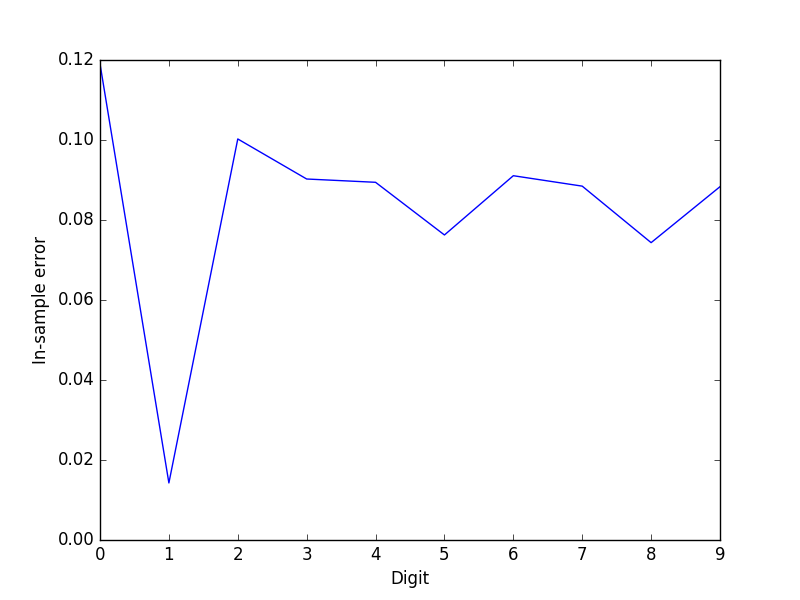
\includegraphics[width=0.65\textwidth]{p2.png}
\caption{In-sample errors of handwriting data}
\end{center}
\end{figure}

\section*{Problem 3} 

\textbf{(A)} - The digit 1 has the lowest in-sample error by far with an error of 0.014.

\section*{Problem 4}

\textbf{(C)} - The total number of support vectors for 0 is 2279 and the total number of support vectors for 1 is 400, so the difference is around 1800.

\section*{Problem 5}

\textbf{(D)} - The number of support vectors does decrease as C increases from 0.001 to 0.1 (from 76 to 34 to 24), however it remains at 24 when C = 1. $E_{out}$ goes up from 0.016 to 0.018 with increasing C. The only answer choice that is true is that when C = 1 we get the lowest $E_{in}$, a value of 0.0032.

\section*{Problem 6}

\textbf{(B)} - In this case, the only answer choice that is correct is that the number of support vectors drops from 76 to 25 when Q increases from 2 to 5. When C = 0.01, $E_{in}$ decreases from 0.0045 to 0.0038. When C = 1 $E_{out}$ increases from 0.0189 to 0.0212. Finally, when C = 0.001, $E_{in}$ is 0.0045 in both cases.

\section*{Problem 7}

\textbf{(B)} - Out of 1000 trials, 0.001 was selected 457 times, while 0.0001, 0.02, 0.1, and 1 were selected 0, 229, 128, and 186 times respectively.

\section*{Problem 8}

\textbf{(C)} - The code finds that using C = 0.001, we get an average $E_{cv}$ value of 0.0047.

\section*{Problem 9}

\textbf{(E)} - The lowest $E_{in}$ occurs when C = $10^6$ which makes sense because this is the largest C we tested. The error in this case is $6.4 * 10^{-4}$.

\section*{Problem 10}

\textbf{(C)} - The lowest $E_{out}$ occurs when C = 100 (actually tied with C = 10, 1000, and $10^5$, but the only answer choice is 100) with an error of 0.0189.

\end{document}
	% line of code telling latex that your document is ending. If you leave this out, you'll get an error
